\documentclass[sn-basic]{sn-jnl}

\usepackage{graphicx}
\usepackage{manyfoot}
\usepackage{textcomp}
\usepackage{amsmath,amssymb}
\usepackage{booktabs}
\usepackage{multirow}
\usepackage{xcolor}
\usepackage{xurl}
\usepackage[title]{appendix}
\graphicspath{{figures/}{../survey/figures/}}
\newcommand{\INR}{INR~}

\raggedbottom

\begin{document}

\title[Home Loans in India Before, During and After COVID-19]{A Study on Home Loans with Special Reference to Mortgage Loans in India: Before, During and After COVID-19}

\author*[1]{\fnm{Harsh} \sur{Raj}}\email{harsh.raj19061999@gmail.com}

\affil*[1]{\orgdiv{Department of Finance and Risk Engineering}, \orgname{New York University Tandon School of Engineering}, \orgaddress{\city{Brooklyn}, \state{NY}, \country{USA}}}

\abstract{\textbf{Purpose:} This study examines how the cost and risk of a home loan in India changed across three periods: before COVID-19 (2016 to February 2020), during the pandemic (March 2020 to March 2022) and after it (April 2022 to 2026), a span in which home loans became linked to the Reserve Bank of India's repo rate.
\textbf{Methods:} The study combines market data for each period, amortisation calculations for a standard \INR 5 million (50 lakh), 20-year loan under each period's rates, tax rules and relief measures, and a survey of 120 borrowers at four groups of lenders, analysed with permutation tests and a Holm adjustment.
\textbf{Results:} Total interest on the same loan ranged from \INR 4.09 million at the 2021 low to \INR 5.91 million at the 2023 peak. A borrower who took a loan at 6.70\% in mid-2021 now faces a loan 7.5 years longer and \INR 3.38 million more interest than planned, while a 2019 borrower came out almost even. Deferring six instalments under the 2020 moratorium added 33 months and about \INR 1.1 million of interest. The tax value of a home loan for salaried owner-occupiers, up to \INR 92,500 a year in 2019-20, has been displaced by the new tax regime. Borrowers were content with rates but not with the process: 88\% found getting a loan time-consuming, with significant differences between lenders.
\textbf{Conclusion:} Repo-linked pricing has transferred interest-rate risk to borrowers, so that when a borrower takes a loan matters more than which lender they choose.}

\keywords{Home loans, Mortgage, External benchmark lending rate, COVID-19 moratorium, Monetary transmission, India}

\pacs[JEL Classification]{G21, G51, R31, E52}

\maketitle

\section{Introduction}\label{sec:intro}

Housing is one of the three basic needs of life, and for most families in India a home is the largest purchase they will ever make. Very few can pay for it outright, so the home loan is the instrument that turns the wish for a house into ownership. A mortgage loan is a loan secured by property: a buyer pledges the home being bought, or an owner pledges an existing property to raise money for another purpose, and the lender holds a claim on the property until the loan is repaid. Since the National Housing Bank was set up in 1988, India's housing finance industry has grown from a small, tightly regulated sector into a competitive market served by public and private banks and housing finance companies (HFCs). By March 2024 outstanding housing loans had reached about \INR 27 lakh crore (\INR 27 trillion), up \INR 10 lakh crore in two years \citep{outlook2024}.

The period since 2016 has tested this market three times over. Before the pandemic, a slowdown in property and a credit squeeze on non-bank lenders coincided with falling interest rates and, from October 2019, a switch to home loans priced off the repo rate \citep{rbi2019eblr}. During the pandemic, a repayment moratorium, loan restructuring and the lowest rates in two decades froze and then revived the market. After it, 2.5 percentage points of rate rises, record home sales and a new round of cuts in 2025 followed in quick succession.

This paper asks three questions. How did the cost of the same home loan differ across the three periods? How did borrowers who lived through the rate cycle fare, given that repo-linked loans pass policy-rate changes through to existing borrowers? And what do borrowers themselves say about getting a loan? It contributes to a literature that largely predates both repo-linked pricing and the pandemic by quantifying, for a standard loan, the effects of the rate cycle, the moratorium and the change in tax rules, and by re-analysing a survey of borrowers with methods suited to small groups.

\section{Literature review}\label{sec:lit}

Earlier Indian studies of housing finance fall into two groups. Studies of the industry describe its structure and the entry of banks into a market once led by HFCs: \citet{kotireddy2011} described the Indian mortgage industry, and \citet{vikkraman2004} and \citet{dhanija2015} traced the growth of HFCs, using LIC Housing Finance as a case. \citet{sangwan2012} and \citet{chauhan2017} compared public and private sector banks and found private banks faster to process loans and public banks cheaper. Studies of borrowers, such as \citet{nazrine2017}, \citet{nalluswamy2012} and \citet{verma2015}, surveyed awareness and satisfaction and found that the interest rate, processing time and documentation shape the choice of lender.

These studies predate two developments that changed what a home loan costs and who bears its risk. The first is the external benchmark: since October 2019, floating-rate retail loans have had to be linked to an external rate, in practice the repo rate, instead of each bank's marginal cost of funds based lending rate (MCLR) \citep{rbi2019eblr}. The second is the pandemic, with its moratorium and restructuring frameworks \citep{paisabazaar2021,rbi2021rf2}. This paper adds to the literature by comparing borrowers' costs across the first full rate cycle, from 2019 to 2026, in which policy-rate changes passed directly into home loans.

\section{Home loans across three periods}\label{sec:eras}

\subsection{Mortgage loans and their pricing}

The main types of mortgage loan in India are home loans (to buy, build or extend a home, typically for up to 30 years and 75--90\% of the property's value), loans against property (an existing property pledged for any purpose, typically 50--70\% of its value, at a higher rate), commercial purchase loans, lease rental discounting (a loan against future rent), second mortgages and reverse mortgages for owners over 60. Secured on property, mortgage loans carry lower rates than personal loans, and individual borrowers pay no penalty for prepaying a floating-rate loan.

A floating-rate home loan has two parts: a benchmark that moves with the market and a spread fixed when the loan is made. Until September 2019 banks priced loans off their own MCLR, through which cuts in the policy rate reached borrowers slowly and only in part. From 1 October 2019 new loans have been linked to the repo rate, so a change reaches the borrower at the next reset, usually within three months \citep{rbi2019eblr}. HFCs still price off their own prime lending rates. Government support has come mainly through the Credit Linked Subsidy Scheme of Pradhan Mantri Awas Yojana (PMAY), which closed to middle-income buyers in March 2021, and PMAY-Urban 2.0, which from 2024 offers first-time buyers with household incomes up to \INR 0.9 million an interest subsidy of up to \INR 180,000 \citep{icicihfc2024}.

\begin{figure}[t]
\centering
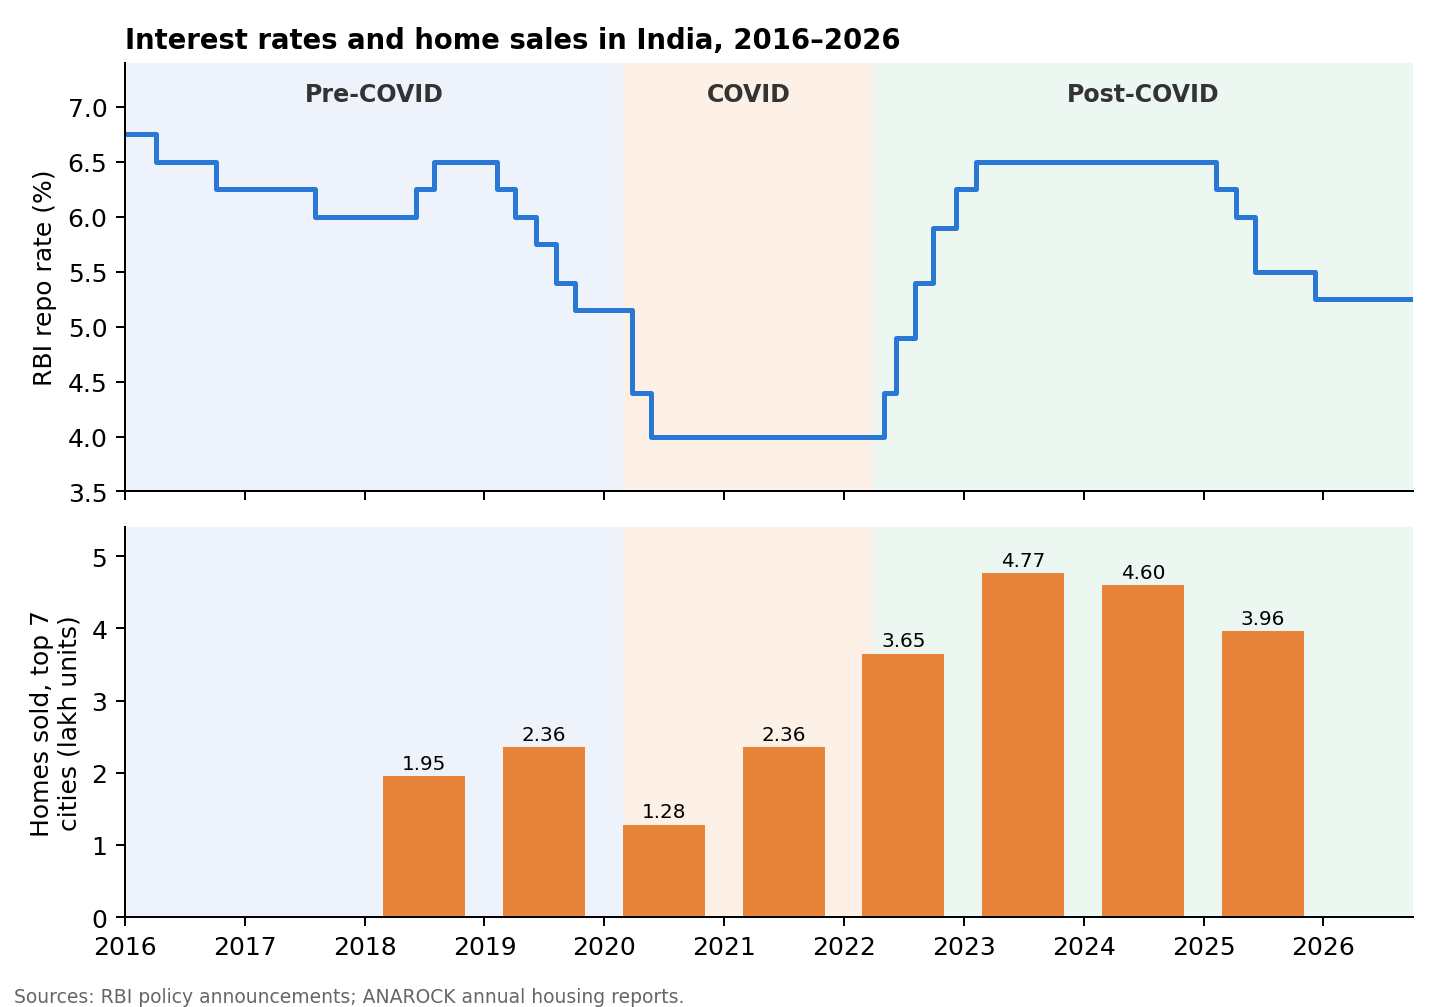
\includegraphics[width=0.95\textwidth]{eras.png}
\caption{The RBI repo rate and annual home sales in the seven largest cities, 2016--2026, with the three periods shaded. Sources: RBI policy announcements \citep{cleartaxrepo}; ANAROCK \citep{anarock2022,tribune2024,mediabrief2025}}\label{fig:eras}
\end{figure}

\subsection{Pre-COVID: 2016 to February 2020}

Home sales in the seven largest cities had peaked at 343,000 units in 2014 and fell to 195,000 in 2018 \citep{anarock2022}, as demonetisation (November 2016), the goods and services tax (July 2017) and the Real Estate (Regulation and Development) Act of 2016 hit developers in quick succession. In September 2018, Infrastructure Leasing \& Financial Services defaulted and lenders stopped rolling over the short-term borrowing of non-bank lenders; Dewan Housing Finance, then one of the largest HFCs, defaulted in 2019. For borrowers, rates were high but falling: the repo rate was cut five times in 2019, from 6.50\% to 5.15\% (Figure~\ref{fig:eras}), but under MCLR pricing SBI home loans still started at about 8.75\% for much of the year \citep{nobroker2025}. Section 80EEA allowed first-time buyers of affordable homes an extra \INR 150,000 interest deduction for loans sanctioned from April 2019 to March 2022. Sales recovered to 236,000 homes in 2019 \citep{anarock2022}.

\subsection{COVID-19: March 2020 to March 2022}

The lockdown from late March 2020 stopped site visits, registrations and construction. The RBI cut the repo rate to 4.40\% on 27 March and to 4.00\% on 22 May 2020, and held it there for two years. Lenders could let borrowers defer instalments falling due from 1 March to 31 August 2020, with interest accruing and added to the loan; under Resolution Framework 1.0 (August 2020) and 2.0 (May 2021), they could reschedule stressed loans, including extending the tenure by up to two years \citep{paisabazaar2021,rbi2021rf2}. Sales fell to 128,000 homes in 2020, the lowest in the period \citep{anarock2022}. The recovery was quick: SBI's rate started at 6.70\% in 2021, Maharashtra cut stamp duty from September 2020 to March 2021, and sales in the first quarter of 2021 were 29\% above a year earlier \citep{bs2021q1}. The 2020 budget also introduced an optional income-tax regime with lower slabs and almost no deductions, including none for a home loan on a self-occupied property.

\subsection{Post-COVID: April 2022 to 2026}

As inflation rose, the RBI raised the repo rate six times between May 2022 and February 2023, from 4.00\% to 6.50\%. Because most loans were now repo-linked, the full 2.5 points reached existing borrowers within months, and SBI's starting rate rose to 9.15\% \citep{navi2023}. Most lenders kept instalments unchanged and lengthened loans, some past the borrower's retirement age; in August 2023 the RBI required lenders to explain resets and let borrowers choose between a higher instalment, a longer tenure or a fixed rate. Sales nonetheless set records: 365,000 homes in 2022, 477,000 in 2023 and 460,000 in 2024, before falling 14\% to 396,000 in 2025 while their value rose to over \INR 6 lakh crore \citep{anarock2022,tribune2024,mediabrief2025}. In July 2023, HDFC Ltd, India's largest HFC, merged into HDFC Bank. In 2025 the RBI cut the repo rate four times, to 5.25\%, and held it there in August 2026 \citep{iifl2026repo}. In September 2026, starting rates ranged from 7.20\% (Punjab National Bank) and 7.25\% (SBI) to 8.35\% (Axis Bank) \citep{urbanmoney2026}. The new tax regime became the default in 2023 and, from 2025, charges no tax on salaries up to \INR 1.275 million \citep{cleartaxslabs}.

\section{Data and methods}\label{sec:methods}

\subsection{Secondary data and loan calculations}

Market data come from RBI policy statements and circulars, lenders' published rates, ANAROCK's housing reports and financial news reports citing official data. All loan calculations use a principal $P$ of \INR 5 million over $n = 240$ monthly instalments. With monthly rate $r = R/1200$ for an annual rate $R$ in per cent, the equated monthly instalment (EMI) is
\begin{equation}
E = \frac{P\,r\,(1+r)^{n}}{(1+r)^{n}-1},\label{eq:emi}
\end{equation}
and the outstanding balance evolves as
\begin{equation}
B_{t} = B_{t-1}\,(1 + r_t) - E_t, \qquad B_0 = P,\label{eq:bal}
\end{equation}
where $r_t$ is the monthly rate in month $t$. For repo-linked loans, $r_t$ equals the repo rate plus a fixed spread, and each RBI decision takes effect in the month after it is announced. Following lenders' default practice, the instalment $E_t$ is held constant when the rate changes, so the tenure adjusts; if the instalment no longer covers the month's interest, it is recalculated to repay the balance over the remaining original term. For the moratorium, deferred instalments are skipped and the month's interest is added to the balance. Income tax follows the rules for a salaried resident under 60 in FY 2019-20 and FY 2026-27, including the standard deduction, the \INR 200,000 cap on interest, the \INR 150,000 limit on principal and other tax-saving investments, the rebates and the 4\% cess; surcharge is excluded. The calculations are implemented in a tested JavaScript module published with the paper.

\subsection{Survey}

The survey was conducted in 2022, as the COVID period ended. 120 home-loan borrowers, 30 each from SBI, ICICI Bank, HDFC and non-bank lenders (NBFCs and HFCs), were reached through personal contact. They included salaried employees, self-employed professionals, business owners and homemakers. The questionnaire covered occupation, age, gender, when the loan was taken, satisfaction, the reason for choosing the lender, the source of information, and views on the rate, processing time, paperwork and terms and conditions.

For each question, a permutation test of the chi-square statistic (20,000 random reassignments of answers across lenders) tests whether lenders differ by more than chance, which is valid for groups of 30 where expected counts are small. Cram\'er's $V$ measures the size of any difference, and Holm's method adjusts the $p$-values for testing 11 questions.

\section{Results}\label{sec:results}

\subsection{The cost of the same loan in each period}

Table~\ref{tab:eras} applies Eq.~(\ref{eq:emi}) to SBI's starting rate in each period. Total interest on the same loan ranged from \INR 4.09 million at the 2021 low to \INR 5.91 million at the 2023 peak, a difference of \INR 1.82 million. By comparison, the gap between the cheapest (7.20\%) and dearest (8.35\%) mainstream lender in September 2026 is worth \INR 0.85 million. In every period, 73--83\% of the first year's payments go to interest.

\begin{table}[h]
\caption{A \INR 5 million, 20-year loan at SBI's starting rate in each period}\label{tab:eras}
\footnotesize
\begin{tabular}{@{}lrrrr@{}}
\toprule
 & Pre-COVID & COVID & Post-COVID peak & Today \\
 & (2019) & (2021) & (2023) & (2026) \\
\midrule
RBI repo rate & 6.50\% $\to$ 5.15\% & 4.00\% & 6.50\% & 5.25\% \\
SBI home-loan rate, from & about 8.75\% & 6.70\% & 9.15\% & 7.25\% \\
Monthly instalment (INR) & 44,186 & 37,870 & 45,470 & 39,519 \\
Total interest (INR million) & 5.60 & 4.09 & 5.91 & 4.48 \\
Interest as \% of the loan & 112\% & 82\% & 118\% & 90\% \\
Homes sold, top 7 cities (thousand) & 236 & 236 & 477 & 396 (2025) \\
\botrule
\end{tabular}
\footnotetext{Sources: rates from \citet{nobroker2025}, \citet{navi2023} and \citet{urbanmoney2026}; sales from ANAROCK \citep{anarock2022,tribune2024,mediabrief2025}; instalments and interest calculated.}
\end{table}

\subsection{Borrowers who lived through the rate cycle}

Two borrowers illustrate how the path of rates after borrowing determines the cost of a repo-linked loan (Table~\ref{tab:cycle}). Borrower A took a loan in October 2019, the month repo-linked loans began, at 8.15\% (the repo rate plus 3.00 points). Their rate fell to 7.00\% during the pandemic, rose to 9.50\% by 2023 and returned to 8.25\% after the 2025 cuts. The low pandemic years let the loan amortise faster, which offset most of the later rises: it ends only 3 months later than planned.

Borrower B took a loan in June 2021 at 6.70\% (the repo rate plus 2.70 points). Their rate rose to 9.20\% by March 2023, when the month's interest of about \INR 37,160 absorbed almost all of the \INR 37,870 instalment and the loan barely amortised. Had rates stayed at the 2023 peak, the loan would have run 541 months, or 45 years. With the 2025 cuts it runs 330 months, 7.5 years longer than planned, and costs \INR 3.38 million more in interest. Borrowers who took the cheapest loans of the pandemic, often first-time buyers, carried the most rate risk.

\begin{table}[h]
\caption{Two \INR 5 million, 20-year repo-linked loans with the instalment held constant}\label{tab:cycle}
\footnotesize
\begin{tabular}{@{}lrr@{}}
\toprule
 & Borrower A & Borrower B \\
\midrule
Loan taken & October 2019 & June 2021 \\
Starting rate (repo + spread) & 8.15\% (5.15 + 3.00) & 6.70\% (4.00 + 2.70) \\
Peak rate & 9.50\% & 9.20\% \\
Rate in 2026 & 8.25\% & 7.95\% \\
Tenure, planned $\to$ actual (months) & 240 $\to$ 243 & 240 $\to$ 330 \\
Extra interest (INR million) & 0.10 & 3.38 \\
Tenure if the 2023 peak had persisted (months) & -- & 541 \\
\botrule
\end{tabular}
\footnotetext{Repo-rate changes applied in the month after each RBI decision, with full pass-through.}
\end{table}

\subsection{The cost of the moratorium}

Applying the moratorium to Borrower A's loan at a constant 8.15\% and deferring all six instalments from March to August 2020 gave the borrower \INR 254,000 of relief at the time. With interest added to the balance and the instalment unchanged afterwards, the loan ends 33 months later and total interest rises by about \INR 1.11 million. The deferred interest is repaid at the end of the loan, where each extra month costs a full instalment. For borrowers who could still pay, the moratorium was an expensive form of credit; it was valuable for those whose incomes had actually stopped.

\subsection{The tax benefit, then and now}

In FY 2019-20 there was one tax regime, and deducting first-year interest and principal on the loan cut a salaried borrower's tax by \INR 61,700 at a salary of \INR 1 million and by \INR 92,500 at \INR 1.5 million or more. In FY 2026-27 the same deductions are available only under the old regime, and the new regime is cheaper even after them: by \INR 41,000 at \INR 1 million (where new-regime tax is nil), \INR 61,500 at \INR 1.5 million and \INR 151,000 at \INR 2.5 million. For most salaried owner-occupiers, a home loan is no longer a reason to choose the old regime.

\subsection{Survey of borrowers}

Table~\ref{tab:survey} and Figure~\ref{fig:survey} report the survey. Borrowers' main complaint was the process, not the price: 88\% found getting a loan time-consuming and 60\% said it needed a lot of paperwork, yet 82\% thought their rate in line with the market and 69\% chose their lender mainly on rate. The survey was taken while rates were at their pandemic lows, which may explain the contentment with price. Lenders differed most on processing time: every ICICI and HDFC borrower found the process time-consuming, against 63\% at SBI, the only difference that remains clear after the Holm adjustment. Satisfaction was high but not deep: 88\% were satisfied or highly satisfied, but only 20\% of SBI borrowers were highly satisfied, against 53\% at HDFC. 53\% learned of their loan online, including 77\% at NBFCs.

The groups also borrowed in different periods. 77\% of SBI borrowers had taken their loan 1--10 years earlier, mostly before the pandemic, while 63\% of HDFC borrowers and half of NBFC borrowers had borrowed in the past year, during the pandemic-era boom in lending. Some differences between lenders may therefore reflect when people borrowed rather than how each lender works.

\begin{table}[h]
\caption{Survey answers by lender ($n = 30$ per lender)}\label{tab:survey}
\footnotesize
\begin{tabular}{@{}lrrrrrrr@{}}
\toprule
Share of borrowers who & SBI & ICICI & HDFC & NBFCs & $p$ & Holm $p$ & $V$ \\
\midrule
found getting the loan time-consuming & 63\% & 100\% & 100\% & 87\% & $<$0.001 & $<$0.001 & 0.32 \\
took the loan in the last year & 20\% & 40\% & 63\% & 50\% & 0.002 & 0.018 & 0.30 \\
said it needed a lot of paperwork & 70\% & 40\% & 50\% & 80\% & 0.007 & 0.063 & 0.32 \\
were highly satisfied & 20\% & 37\% & 53\% & 37\% & 0.020 & 0.162 & 0.23 \\
learned about the loan online & 27\% & 57\% & 50\% & 77\% & 0.028 & 0.198 & 0.23 \\
are business owners & 37\% & 20\% & 20\% & 50\% & 0.039 & 0.235 & 0.22 \\
are women & 13\% & 23\% & 30\% & 43\% & 0.080 & 0.399 & 0.24 \\
think the rate is in line with the market & 87\% & 77\% & 93\% & 70\% & 0.109 & 0.436 & 0.23 \\
chose mainly on interest rate & 70\% & 67\% & 63\% & 77\% & 0.374 & 1.000 & 0.17 \\
are aged 31--40 & 53\% & 57\% & 53\% & 53\% & 0.835 & 1.000 & 0.12 \\
are aware of all terms and conditions & 67\% & 70\% & 77\% & 73\% & 0.902 & 1.000 & 0.08 \\
\botrule
\end{tabular}
\footnotetext{$p$: permutation test of the chi-square statistic over all answer categories, 20,000 reassignments. Holm $p$: adjusted for 11 questions. $V$: Cram\'er's $V$.}
\end{table}

\begin{figure}[h]
\centering
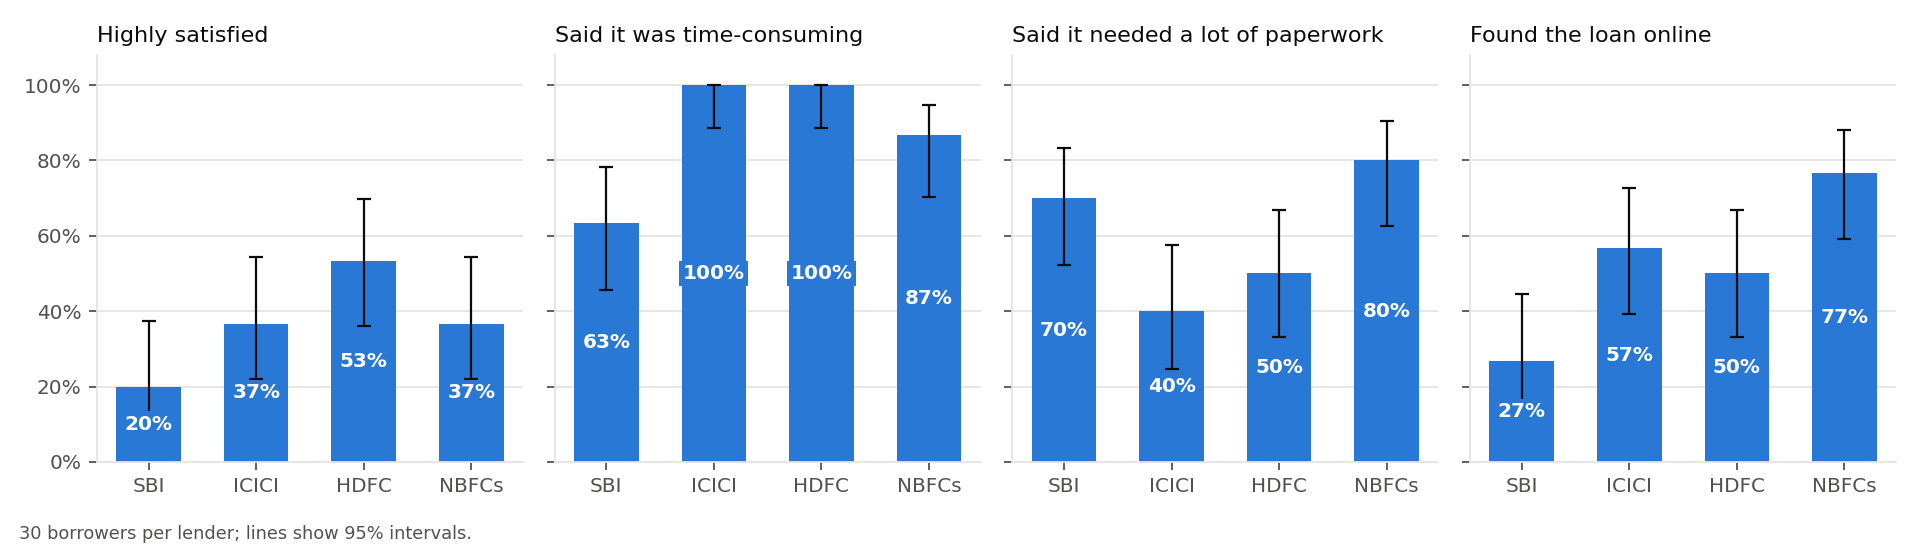
\includegraphics[width=0.95\textwidth]{by_lender.png}
\caption{Selected survey answers by lender, with 95\% Wilson confidence intervals}\label{fig:survey}
\end{figure}

\section{Discussion}\label{sec:discussion}

The findings point to one conclusion: under repo-linked pricing, the timing of a loan matters more than the lender. The cost of an identical loan varied by \INR 1.82 million across the cycle, twice the spread between the cheapest and dearest lenders today, and borrowers who locked in the pandemic lows took the most risk because the lower their starting rate, the closer a rise brought the interest to their instalment. The default practice of extending tenures hid this risk from borrowers until their loans ran decades longer than planned. The moratorium, designed as relief, was costly for borrowers who used it without needing it, and the move to the new tax regime has removed a benefit that once made borrowing cheaper for salaried owner-occupiers.

For borrowers, the implications are practical: compare the spread over the repo rate rather than the headline rate, since the spread is fixed for the life of the loan and one percentage point costs about \INR 0.75 million at current rates on a \INR 5 million, 20-year loan; raise the instalment rather than extend the tenure when rates rise, and check that cuts are passed on; use a moratorium only when income has actually stopped; prepay early where possible, since on a loan at 7.55\% \INR 500,000 prepaid in year 3 saves \INR 1.09 million of interest against \INR 0.19 million in year 15; and compare both tax regimes before choosing the old one for the loan. For lenders, the survey shows that processing time and paperwork are where borrowers see the biggest differences, that the digital processes adopted during the pandemic should become the norm, and that rate resets need to be explained clearly.

The study has limitations. The survey is small and not random: 30 borrowers per lender can reveal only large differences, and taken in 2022 it reflects views before the rate rises of 2022--23. Rates are advertised starting rates, and before October 2019 many loans were priced off MCLR rather than the repo rate. The loan examples assume full, immediate pass-through of repo changes and a fixed spread, whereas real resets occur quarterly and vary by lender. The tax examples cover salaried residents under 60 and exclude surcharge.

\section{Conclusion}\label{sec:conclusion}

Between 2019 and 2026 the Indian home-loan market went through a full cycle in seven years: falling rates and a shift to repo-linked pricing; a pandemic that froze the market and then revived it with the lowest rates in two decades; the sharpest rate rises in a decade, with record sales regardless; and a new round of cuts. Because loans are now linked to the repo rate, borrowers feel these cycles directly, in the length of their loans if not in their instalments. The fundamentals of housing demand, a young population, rising incomes and the move to nuclear families, have not changed, but the risk that a borrower's rate will move has shifted from the lender to the borrower. The best protection is to borrow with room to raise the instalment, to prepay early, and to treat the lowest rates of any cycle as temporary.

\backmatter

\bmhead{Acknowledgements}
The author thanks the borrowers who took part in the survey.

\section*{Declarations}

\begin{itemize}
\item \textbf{Funding:} No funding was received for this study.
\item \textbf{Competing interests:} The author has no competing interests to declare.
\item \textbf{Ethics approval and consent to participate:} Participation in the survey was voluntary, and only aggregate answer counts were retained; no personal identifying information is reported.
\item \textbf{Data availability:} The survey counts, market data and loan calculations are available at \url{https://github.com/harsh-github007/Mortgage-Loans-in-India}.
\item \textbf{Code availability:} The loan and tax calculations (with tests) and the survey analysis script are available in the same repository, and the calculations can be reproduced interactively at \url{https://harsh-github007.github.io/Mortgage-Loans-in-India/}.
\item \textbf{Author contributions:} Harsh Raj designed the study, collected and analysed the data and wrote the manuscript.
\end{itemize}

\bibliography{references}

\end{document}
